%%%%%%%%%%%%%%%%%%%%%%%%%%%%%%%%%%%%%%%%%%%%%%%%%%%%%%%%%%%%%%%%%%%%%%%%%%%%%%%%%%%%%%%%%%%%%%%%%%%%
%	chap02 (データの整理)
%===================================================================================================
%	AUTHOR	H. NAKAJIMA
%	DATE	2025/01
%===================================================================================================
%	EDIT HISTORY
%	DATE		NAME			OVERVIEW
%---------------------------------------------------------------------------------------------------
%	2025/01		H. NAKAJIMA		Create new
%%%%%%%%%%%%%%%%%%%%%%%%%%%%%%%%%%%%%%%%%%%%%%%%%%%%%%%%%%%%%%%%%%%%%%%%%%%%%%%%%%%%%%%%%%%%%%%%%%%%

{
	\centering
	{\textbf{第 2 章 \indent データの整理}} \\
}

{\textbf{\S 2.1 \indent 1 次元のデータ}}
\basic
\begin{qenumerate}
	\item{
		累積度数分布表は以下のようになる.
		\begin{table}[H]
			\centering
			\begin{tabular}{c|c|c} \hline
				階級値 (cm) & 累積度数 & 累積相対度数 \\ \hline
				164 &  5 & 0.125 \\
				168 & 13 & 0.325 \\
				172 & 25 & 0.625 \\
				176 & 31 & 0.775 \\
				180 & 36 & 0.900 \\
				184 & 40 & 1.000 \\ \hline
			\end{tabular}
		\end{table}
	}
	\item{
		ヒストグラムと度数折れ線は以下のようになる.
		\begin{figure}[H]
			\centering
			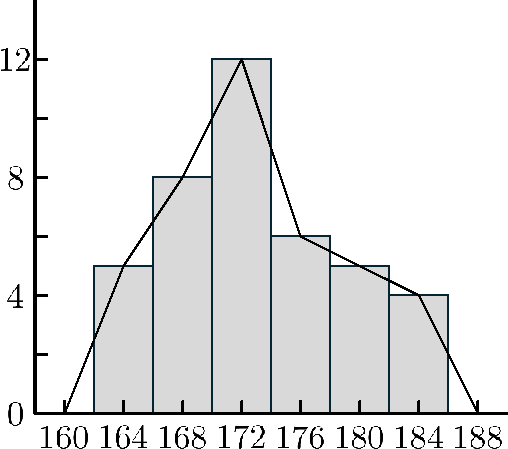
\includegraphics[scale = 0.5]{./figure/73.pdf}
		\end{figure}
	}
	\item{
		求める平均 $\overline{x}$ は
		\begin{align}
			\overline{x} &= \frac{5\cdot 164 \! + \! 8 \! \cdot \! 168 \! + \! 12 \! \cdot \! 172 \! + \! 6 \! \cdot \! 176 \! + \! 5 \! \cdot \! 180 \! + \! 4 \! \cdot \! 184}{40} \\
				&= \red{173}.
		\end{align}
	}
	\item{
		変換後のデータは
		\begin{align}
			u: \red{-12}, \quad \red{11}, \quad \red{-4}, \quad \red{15}, \quad \red{18}, \quad \red{-18}, \quad \red{16}
		\end{align}
		である.
		またデータの平均は, $\overline{u} = \dfrac{\overline{x} - 30}{0.01}$ より
		\begin{align}
			\overline{x} &= 0.01\overline{u} + 30 \\
				&= 0.01\cdot\frac{-12 \! + \! 11 \! + \! (-4) \! + \! 15 \! + \! 18 \! + \! (-18) \! + \! 16}{7} + 30 \\
				&\simeq 0.01\cdot 3.7 + 30 \\
				&\simeq \red{30.04}. 
		\end{align}
	}
	\item{
		\begin{enumerate}
			\item{
				平均値 $\overline{x}$ は
				\begin{align}
					\overline{x} = \frac{1 + 1 + 2 + 3 + 4 + 5 + 5 + 7 + 9 + 10}{10} = \red{4.7}.
				\end{align}
				データ数が偶数だから, 中央値は
				\begin{align}
					\frac{4 + 5}{2} = \red{4.5}.
				\end{align}
			}
			\item{
				平均値 $\overline{x}$ は
				\begin{align}
					\overline{x} = \frac{1 + 1 + 2 + 3 + 4 + 5 + 6 + 7 + 9 + 10 + 18}{11} = \red{6}.
				\end{align}
				データ数が奇数だから, 中央値は\red{5}.
			}
		\end{enumerate}
	}
	\item{
		度数が一番大きい階級は 60--65 だから, 最頻値は
		\begin{align}
			\frac{60 + 65}{2} = \red{62.5}.
		\end{align}
		データ数が 45 だから, 中央値は順に並んだデータの 23 番目のデータである.
		以下の累積度数分布表において, 累積度数が 23 になる階級は \red{55--60}.
		\begin{table}[H]
			\centering
			\begin{tabular}{c|c|c} \hline
				階級 (kg) & 度数 & 累積度数 \\ \hline
				40--45 &  2 &  2 \\
				45--50 &  4 &  6 \\
				50--55 & 12 & 18 \\
				\textbf{55--60} &  9 & \textbf{27} \\
				60--65 & 13 & 40 \\
				65--70 &  2 & 42 \\
				70--75 &  0 & 42 \\
				75--80 &  3 & 45 \\ \hline
			\end{tabular}
		\end{table}
	}
	\item{
		得点の最大値は 8, 最小値は 2 であるから, 範囲は $8 - 2 = \red{6}$.
		得点の平均 $\overline{x}$ は
		\begin{align}
			\overline{x} = \frac{4 + 6 + 2 + 8 + 3 + 6 + 5 + 3 + 6 + 7 + 5 + 8}{12} = \red{5.25}.
		\end{align}
		得点の分散 $v_{x}$ は
		\begin{align}
			v_{x} = \frac{(4 - 5.25)^{2} + \cdots + (8 - 5.25)^{2}}{12} \simeq 3.5208
		\end{align}
		であるから, 標準偏差 $s_{x}$ は
		\begin{align}
			s_{x} = \sqrt{v_{x}} = \sqrt{3.5208} = \red{1.876}.
		\end{align}
	}
	\item{
		気温の平均 $\overline{x}$ は
		\begin{align}
			\overline{x} &= \frac{19.6 + \cdots + 19.1}{10} = \red{20.65}.
		\end{align}
		気温の分散 $v_{x}$ は
		\begin{align}
			v_{x} = \frac{(19.6 - 20.65)^{2} + (19.1 - 20.65)^{2}}{10} = 7.8525
		\end{align}
		であるから, 標準偏差 $s_{x}$ は
		\begin{align}
			s_{x} = \sqrt{v_{x}} = \sqrt{7.8525} \simeq \red{2.802}.
		\end{align}
	}
	\item{
		女子学生の身長の平均 $\overline{x}$ は
		\begin{align}
			\overline{x} = \frac{4\cdot 146 + \cdots 2\cdot 174}{100} = \red{159.36}.
		\end{align}
		女子学生の身長の分散 $v_{x}$ は
		\begin{align}
			v_{x} = \frac{4\cdot (146 - 159.36)^{2} + 2\cdot (174 - 159.36)^{2}}{100} = 37.1904
		\end{align}
		であるから, 標準偏差 $s_{x}$ は
		\begin{align}
			s_{x} = \sqrt{v_{x}} = \sqrt{37.1904} \simeq \red{6.098}.
		\end{align}
	}
\end{qenumerate}

%\vspace{\baselineskip}
\check
\begin{qenumerate}
	\item{
		\begin{enumerate}
			\item{
				累積度数分布表は以下のようになる.
				\begin{table}[H]
					\centering
					\begin{tabular}{c|c|c} \hline
						階級値 (cm) & 累積度数 & 累積相対度数 \\ \hline
						157.5 &  1 & 0.025 \\
						162.5 &  6 & 0.150 \\
						167.5 & 17 & 0.425 \\
						172.5 & 31 & 0.775 \\
						177.5 & 38 & 0.950 \\
						182.5 & 40 & 1.000 \\ \hline
					\end{tabular}
				\end{table}
			}
			\item{
				ヒストグラムと度数折れ線は以下のようになる.
				\begin{figure}[H]
					\centering
					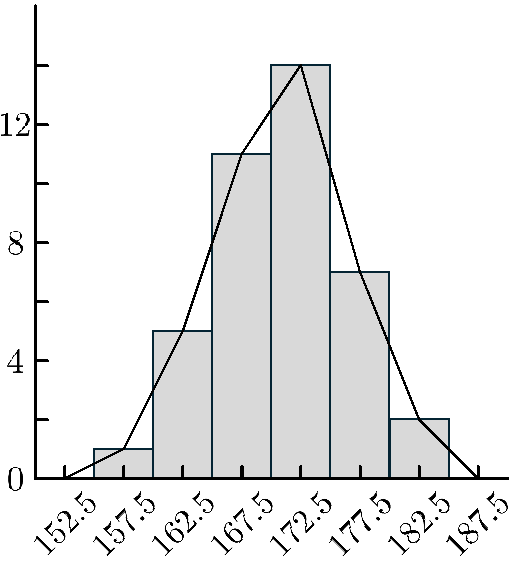
\includegraphics[scale = 0.5]{./figure/81.pdf}
				\end{figure}
			}
			\item{
				身長の平均 $\overline{x}$ は
				\begin{align}
					\overline{x} = \frac{1\cdot 157.5 + \cdots + 2\cdot 182.5}{40} = \red{170.9}.
				\end{align}
			}
		\end{enumerate}
	}
	\item{
		\begin{enumerate}
			\item{
				変量 $u$ のデータは
				\begin{align}
					u: \red{5}, \quad \red{2}, \quad \red{5}, \quad \red{4}, \quad \red{6}, \quad \red{5}, \quad \red{3}, \quad \red{2}
				\end{align}
				であり, これらの平均 $\overline{u}$ は
				\begin{align}
					\overline{u} = \frac{5 + 2 + 5 + 4 + 6 + 5 + 3 + 2}{8} = \red{4}.
				\end{align}
			}
			\item{
				鉛筆の重さの平均 $\overline{x}$ は, $\overline{u} = \dfrac{\overline{x} - 7.4}{0.01}$ より
				\begin{align}
					\overline{x} &= 0.01\overline{u} + 7.4 = 0.01\cdot 4 + 7.4 = \red{7.44}.
				\end{align}
			}
		\end{enumerate}
	}
	\item{
		\begin{enumerate}
			\item{
				台風の発生件数の平均 $\overline{x}$ は
				\begin{align}
					\overline{x} = \frac{21 + \cdots + 23}{10} = \red{26.1}.
				\end{align}
				また, データを昇順に並べると
				\begin{align}
					21\quad 23\quad 23\quad 25\quad 26\quad 27\quad 27\quad 29\quad 29\quad 31
				\end{align}
				となるから, 中央値は
				\begin{align}
					\frac{26 + 27}{2} = \red{26.5}.
				\end{align}
			}
			\item{
				(1) で昇順に並べたデータより, 範囲は $31 - 21 = \red{10}$.
				分散 $v_{x}$ は
				\begin{align}
					v_{x} = \frac{(21 - 26.1)^{2} + \cdot + (31 - 26.1)^{2}}{10} = \red{8.89}.
				\end{align}
				標準偏差 $s_{x}$ は
				\begin{align}
					s_{x} = \sqrt{v_{x}} = \sqrt{8.89} \simeq \red{2.982}.
				\end{align}
			}
		\end{enumerate}
	}
	\item{
		\begin{enumerate}
			\item{
				気温の平均 $\overline{x}$ は
				\begin{align}
					\overline{x} = \frac{5.3 + \cdots + 7.1}{12} \simeq \red{17.6}.
				\end{align}
				また, データを昇順に並べると
				\begin{align}
					&5.3\quad 7.1\quad 8.8\quad 10.6\quad 10.9\quad 16.3 \\
					&20.3\quad 22.8\quad 24.6\quad 26.8\quad 28.5\quad 29.1
				\end{align}
				となるから, 中央値は
				\begin{align}
					\frac{16.3 + 20.3}{2} = \red{18.3}.
				\end{align}
			}
			\item{
				(1) で昇順に並べたデータより, 範囲は $29.1 - 5.3 = \red{23.8}$.
				分散 $v_{x}$ は
				\begin{align}
					v_{x} = \frac{(5.3 - 17.6)^{2} + \cdot + (29.1 - 17.6)^{2}}{10} \simeq \red{71.13}.
				\end{align}
				標準偏差 $s_{x}$ は
				\begin{align}
					s_{x} = \sqrt{v_{x}} = \sqrt{71.13} \simeq \red{8.434}.
				\end{align}
			}
		\end{enumerate}
	}
	\item{
		\begin{enumerate}
			\item{
				度数が一番大きい階級は 170--175 だから, 最頻値は
				\begin{align}
					\frac{170 - 175}{2} = \red{172.5}.
				\end{align}
			}
			\item{
				データ数が 40 だから, 中央値は順に並んだデータの 20 番目のデータである.
				{\textbf{81}} (1) の累積度数分布において, 累積度数が 20 になる階級は \red{170--175}.
			}
			\item{
				{\textbf{81}} (3) より身長の平均は 170.9 だから, 身長の分散 $v_{x}$ は
				\begin{align}
					v_{x} &= \frac{1\cdot (157.5 - 170.9)^{2} + \cdots + 2\cdot (182.5 - 170.9)^{2}}{40} \\
						&\simeq \red{31.73}.
				\end{align}
				分散 $s_{x}$ は
				\begin{align}
					s_{x} = \sqrt{v_{x}} = \sqrt{31.73} \simeq \red{5.633}.
				\end{align}
			}
		\end{enumerate}
	}
	\item{
		通学時間の平均 $\overline{x}$ は
		\begin{align}
			\overline{x} &= \frac{1\cdot 5 + \cdots + 5\cdot 75}{80} \simeq \red{49.1}.
		\end{align}
		通学時間の分散 $v_{x}$ は
		\begin{align}
			v_{x} &= \frac{1\cdot (5 - 49.1)^{2} + \cdot + 5\cdot (75 - 49.1)^{2}}{80} = 211.735
		\end{align}
		であるから, 標準偏差 $s_{x}$ は
		\begin{align}
			s_{x} = \sqrt{v_{x}} = \sqrt{211.735} = \red{14.891}.
		\end{align}
	}
\end{qenumerate}

%\vspace{\baselineskip}
\stepup
\begin{qenumerate}
	\item{
		\begin{enumerate}
			\item{
				変量 $u$ のデータは
				\begin{align}
					u: \red{7}&, \quad \red{1}, \quad \red{3}, \quad \red{16}, \quad \red{8}, \quad \red{3}, \quad \red{10}, \quad \red{1}, \quad \red{11}, \\
						 \red{6}&, \quad \red{13}, \quad \red{5}, \quad \red{18}, \quad \red{16}, \quad \red{0}, \quad \red{11}, \quad \red{3}, \quad \red{9}
				\end{align}
				である.
			}
			\item{
				Sturges の公式より
				\begin{align}
					1 + \frac{\log{18}}{\log{2}} \simeq 5.17
				\end{align}
				となるから, 階級の数は 5 とする.
				また, 階級の幅はデータの範囲を階級の数で割って
				\begin{align}
					\frac{18 - 0}{5} = 3.6
				\end{align}
				となるから, 階級の幅は 4 とする.
				以上の条件から作られる度数分布表は以下のようになる.
				\begin{table}[H]
					\centering
					\begin{tabular}{c|c|c} \hline
						階級 & 階級値 & 度数 \\ \hline
						0 以上 4 未満   & 2 & 6 \\
						4 以上 8 未満   &  6 & 3 \\
						8 以上 12 未満  & 10 & 5 \\
						12 以上 16 未満 & 14 & 1 \\
						16 以上 20 未満 & 18 & 3 \\ \hline
						               & 計 & 18 \\ \hline
					\end{tabular}
				\end{table}
			}
			\item{
				ヒストグラムは以下のようになる.
				\begin{figure}[H]
					\centering
					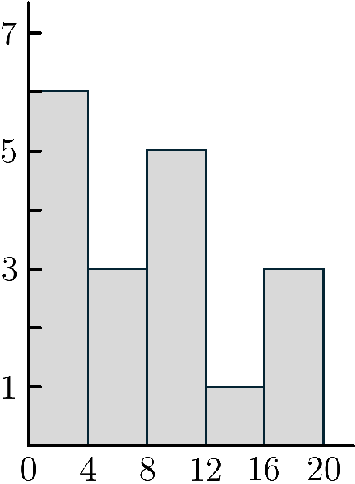
\includegraphics[scale = 0.5]{./figure/87.pdf}
				\end{figure}
			}
		\end{enumerate}
	}
	\item{
		5 歳の身長のデータを $x$, 17 歳の身長のデータを $y$ とすると, これらの平均 $\overline{x}$, $\overline{y}$ は
		\begin{gather}
			\overline{x} = \frac{115.5 + \cdots + 111.0}{10} = 110.19, \\
			\overline{y} = \frac{176.1 + \cdots + 170.6}{10} = 171.7
		\end{gather}
		である.
		また, これらの標準偏差 $s_{x}$, $s_{y}$ は
		\begin{align}
			s_{x} &= \sqrt{\frac{(115.5 - 110.19)^{2} + \cdots + (111.0 - 110.19)^{2}}{10}} \\
				&= \sqrt{12.6929} \simeq 3.563, \\
			s_{y} &= \sqrt{\frac{(176.1 - 171.7)^{2} + \cdots + (170.6 - 171.7)^{2}}{10}} \\
				&= \sqrt{17.2} \simeq 4.147
		\end{align}
		である.
		したがって, 5 歳の身長のデータの変動係数は
		\begin{align}
			\frac{s_{x}}{\overline{x}} = \frac{3.563}{110.19} \simeq \red{0.032}, 
		\end{align}
		17 歳の身長データの変動係数は
		\begin{align}
			\frac{s_{y}}{\overline{y}} = \frac{4.147}{171.7} \simeq \red{0.024}.
		\end{align}
	}
	\item{
		数学の得点のデータを $x$, 英語の得点のデータを $y$ とすると, これらの平均 $\overline{x}$, $\overline{y}$ は
		\begin{gather}
			\overline{x} = \frac{0\cdot 5 + \cdots + 0\cdot 95}{50} = 51.4, \\
			\overline{y} = \frac{0\cdot 5 + \cdots + 5\cdot 95}{50} = 64.6
		\end{gather}
		である.
		また, これらの標準偏差 $s_{x}$, $s_{y}$ は
		\begin{align}
			s_{x} &= \sqrt{\frac{0\cdot (5 - 51.4)^{2} + \cdots + 0\cdot (95 - 51.4)^{2}}{50}} \\
				&= \sqrt{255.04} \simeq 15.97, \\
			s_{y} &= \sqrt{\frac{0\cdot (5 - 64.6)^{2} + \cdots + 5\cdot (95 - 64.6)^{2}}{50}} \\
				&= \sqrt{283.84} \simeq 16.85
		\end{align}
		である.
		したがって, 数学の得点のデータの変動係数は
		\begin{align}
			\frac{s_{x}}{\overline{x}} = \frac{15.97}{51.4} \simeq \red{0.311}, 
		\end{align}
		英語の得点のデータの変動係数は
		\begin{align}
			\frac{s_{y}}{\overline{y}} = \frac{16.85}{64.6} \simeq \red{0.261}.
		\end{align}
	}
\end{qenumerate}

%\vspace{\baselineskip}
{\textbf{\S 2.2 \indent 2 次元のデータ}}
\basic
\begin{qenumerate}
	\item{
		数学の得点の平均 $\overline{x}$, 英語の得点の平均 $\overline{y}$ は
		\begin{align}
			\overline{x} &= \frac{8 + 4 + 6 + 5 + 7 + 8 + 4 + 2}{8} = 5.5, \\
			\overline{y} &= \frac{5 + 6 + 4 + 6 + 4 + 3 + 7 + 9}{8} = 5.5
		\end{align}
		である.
		また, 標準偏差 $s_{x}$, $s_{y}$ は
		\begin{align}
			s_{x} &= \sqrt{\frac{(8 - 5.5)^{2} + \cdots + (2 - 5.5)^{2}}{8}} \\
				&= \sqrt{4} = 2, \\
			s_{y} &= \sqrt{\frac{(5 - 5.5)^{2} + \cdots + (9 - 5.5)^{2}}{8}} \\
				&= \sqrt{3.25}
		\end{align}
		である.
		さらに, $x$ と $y$ の共分散 $s_{xy}$ は
		\begin{align}
			s_{xy} &= \frac{(8 - 5.5)(5 - 5.5) + \cdots + (2 - 5.5)(9 - 5.5)}{8} \\
				&= \frac{(-1.25) + \cdots + (-12.25)}{8} = -3.25
		\end{align}
		である.
		以上より, 相関係数 $r$ は
		\begin{align}
			r &= \frac{s_{xy}}{s_{x}s_{y}} = -\frac{3.25}{2\cdot \sqrt{3.25}} \simeq \red{-0.901}
		\end{align}
		散布図は以下のようになる.
		\begin{figure}[H]
			\centering
			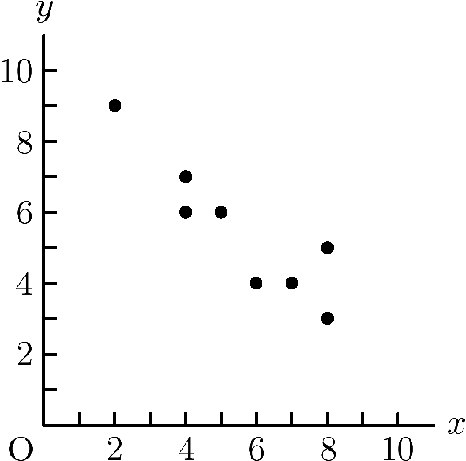
\includegraphics[scale = 0.5]{./figure/90.pdf}
		\end{figure}
	}
	\item{
		年齢の平均 $\overline{x}$, 血圧の平均 $\overline{y}$ は
		\begin{align}
			\overline{x} &= \frac{36 + \cdots + 73}{10} = 54.8, \\
			\overline{y} &= \frac{117 + \cdots + 158}{10} = 138.2
		\end{align}
		である.
		また, 標準偏差 $s_{x}$, $s_{y}$ は
		\begin{align}
			s_{x} &= \sqrt{\frac{(36 - 54.8)^{2} + \cdots + (73 - 54.8)^{2}}{10}} \\
				&= \sqrt{175.56}, \\
			s_{y} &= \sqrt{\frac{(117 - 138.2)^{2} + \cdots + (158 - 138.2)^{2}}{10}} \\
				&= \sqrt{140.56}
		\end{align}
		である.
		さらに, $x$ と $y$ の共分散 $s_{xy}$ は
		\begin{align}
			s_{xy} &= \frac{1}{10}\cdot[(36 - 54.8)(117 - 138.2) + \cdots \\
				&\quad\quad\quad\quad\quad\quad\quad + (73 - 54.8)(158 - 138.2)] \\
				&= \frac{398.56 + \cdots + 360.36}{10} = 150.04
		\end{align}
		である.
		以上より, 相関係数 $r$ は
		\begin{align}
			r &= \frac{s_{xy}}{s_{x}s_{y}} = -\frac{150.04}{\sqrt{175.56}\cdot \sqrt{140.56}} \simeq \red{0.955}
		\end{align}
		散布図は以下のようになる.
		\begin{figure}[H]
			\centering
			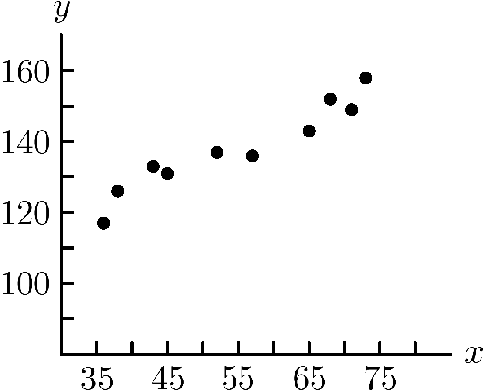
\includegraphics[scale = 0.5]{./figure/91.pdf}
		\end{figure}
	}
	\item{
		\begin{enumerate}
			\item{
				気温の平均 $\overline{x}$, アイスの売上個数の平均 $\overline{y}$ は
				\begin{align}
					\overline{x} &= \frac{0 + 5 + 10 + 15 + 20 + 25 + 30}{7} = 15, \\
					\overline{y} &= \frac{2 + 4 + 7 + 15 + 23 + 28 + 33}{7} = 16
				\end{align}
				である.
				また, 気温の標準偏差 $s_{x}$ は
				\begin{align}
					s_{x} &= \sqrt{\frac{(0 - 15)^{2} + \cdots + (30 - 15)^{2}}{7}} = 10
				\end{align}
				である.
				さらに, 気温とアイスの売り上げ個数の共分散 $s_{xy}$ は
				\begin{align}
					s_{xy} &= \frac{(0 - 15)(2 - 16) + \cdots + (30 - 15)(33 - 16)}{7} \\
						&= \frac{785}{7}
				\end{align}
				である.
				$y$ の $x$ への回帰直線の方程式を
				\begin{align}
					y=ax + b\quad (a, b\in\mathbb{R})
				\end{align}
				とおき, $s_{x}$, $s_{xy}$ から $a$, $b$ を定めると
				\begin{gather}
					a = \frac{s_{xy}}{{s_{x}}^{2}}, \\
					b = \overline{y} - a\overline{x}
				\end{gather}
				より
				\begin{gather}
					a = \frac{785}{7}\cdot \frac{1}{10^{2}} = \frac{157}{140} \simeq 1.12, \\
					b = 16 - \frac{157}{140}\cdot 15 \simeq -0.82.
				\end{gather}
				すなわち, 求める方程式は
				\begin{align}
					\red{y = 1.12x - 0.82}.
				\end{align}
			}
			\item{
				(1) で求めた方程式に $x = 35$ を代入すると
				\begin{align}
					y = 1.12\cdot 35 - 0.82 = 38.38 \simeq 38
				\end{align}
				より, \red{38 個}.
			}
		\end{enumerate}
	}
	\item{
		$x$, $y$ の平均 $\overline{x}$, $\overline{y}$ は
		\begin{align}
			\overline{x} &= \frac{0.8 + 2.7 + 6.1 + 4.6 + 7.3 + 1.5 + 2.3 + 3.2}{8} \\
				&= 3.5625, \\
			\overline{y} &= \frac{11.1 \! + \! 13.1 \! + \! 18.0 \! + \! 17.0 \! + \! 19.3 \! + \! 12.0 \! + \! 14.1 \! + \! 14.8}{8} \\
				&= 14.925
		\end{align}
		である.
		また, $x$ の標準偏差 $s_{x}$ は
		\begin{align}
			s_{x} &= \sqrt{\frac{(0.8 - 3.625)^{2} + \cdots + (3.2 - 3.5625)^{2}}{8}} \\
				&\simeq 2.117
		\end{align}
		である.
		さらに, $x$, $y$ の共分散 $s_{xy}$ は
		\begin{align}
			s_{xy} &= \frac{1}{8}\cdot [(0.8 - 3.5625)(11.1 - 14.925) + \cdots \\
				&\quad\quad\quad\quad\quad\quad\quad + (3.2 - 3.5625)(14.8 - 14.925)] \\
				&\simeq 5.696
		\end{align}
		である.
		$y$ の $x$ への回帰直線の方程式を
		\begin{align}
			y=ax + b\quad (a, b\in\mathbb{R})
		\end{align}
		とおき, $s_{x}$, $s_{xy}$ から $a$, $b$ を定めると
		\begin{gather}
			a = \frac{s_{xy}}{{s_{x}}^{2}} = \frac{5.696}{\sqrt{2.117}^{2}} \simeq 1.27, \\
			b = \overline{y} - a\overline{x} = 14.925 - 1.271\cdot 3.5625 \simeq 10.40.
		\end{gather}
		すなわち, 求める方程式は
		\begin{align}
			\red{y = 1.27x + 10.40}.
		\end{align}
	}
	\item{
		\begin{enumerate}
			\item{
				身長の平均 $\overline{x}$, 運動靴のサイズの平均 $\overline{y}$ は
				\begin{gather}
					\overline{x} = \frac{164 + \cdots + 166}{10} = 172.3, \\
					\overline{y} = \frac{24.5 + \cdots + 27.0}{10} = 27.1
				\end{gather}
				である.
				また, 身長の標準偏差 $s_{x}$ は
				\begin{align}
					s_{x} &= \sqrt{\frac{(164 - 172.3)^{2} + \cdots + (166 - 172.3)^{2}}{10}} \\
						&= \sqrt{31.61}
				\end{align}
				である.
				さらに, 身長と運動靴のサイズの共分散 $s_{xy}$ は
				\begin{align}
					s_{xy} &= \frac{1}{10}\cdot[(164 - 172.3)(24.5 - 27.1) + \cdots \\
						&\quad\quad\quad\quad\quad\quad\quad (166 - 172.3)(27.0 - 27.1)] \\
						&= 9.27
				\end{align}
				である.
				$y$ の $X$ への回帰直線の方程式を
				\begin{align}
					y = ax + b\quad (a, b\in\mathbb{R})
				\end{align}
				とおき, $s_{x}$, $s_{xy}$ から $a$, $b$ を定めると
				\begin{gather}
					a = \frac{s_{xy}}{{s_{x}}^{2}} = \frac{9.27}{\sqrt{31.61}^{2}} \simeq 0.29 \\
					b = \overline{y} - a\overline{x} = 27.1 - \frac{9.27}{31.61}\cdot 172.3 = -23.43.
				\end{gather}
				すなわち, 求める方程式は
				\begin{align}
					\red{y = 0.29x - 23.43}.
				\end{align}
			}
			\item{
				(1) で求めた方程式に $x = 180$ を代入すると
				\begin{align}
					y = 0.29\cdot 180 - 23.43 = 28.77 \simeq 29
				\end{align}
				より, \red{29.0 cm}.
			}
		\end{enumerate}
	}
\end{qenumerate}

%\vspace{\baselineskip}
\check
\begin{qenumerate}
	\item{
		表の空欄を埋めると以下のようになる.
		\begin{table}[H]
			\centering
			\begin{tabular}{r|c|c|c|c|c|} \cline{2-6}
				& $x_{i}$ & $y_{i}$ & $x_{i}^{2}$ & $y_{i}^{2}$ & $x_{i}y_{i}$ \\ \cline{2-6}
				&  1 &  4 & \red{  1} & \red{ 16} & \red{ 4} \\
				& 10 &  9 & \red{100} & \red{ 81} & \red{90} \\
				&  7 &  7 & \red{ 49} & \red{ 49} & \red{49} \\
				&  6 &  8 & \red{ 36} & \red{ 64} & \red{48} \\
				&  8 &  9 & \red{ 64} & \red{ 81} & \red{72} \\
				&  9 &  8 & \red{ 81} & \red{ 64} & \red{72} \\
				&  2 &  5 & \red{  4} & \red{ 25} & \red{10} \\
				&  3 &  7 & \red{  9} & \red{ 49} & \red{21} \\
				&  8 & 10 & \red{ 64} & \red{100} & \red{80} \\
				&  7 &  6 & \red{ 49} & \red{ 36} & \red{42} \\ \cline{2-6}
				合計 & \red{61} & \red{73} & \red{457} & \red{565} & \red{488} \\ \cline{2-6}
			\end{tabular}
		\end{table}
		\begin{enumerate}
			\item{
				表より, 平均 $\overline{x}$, $\overline{y}$ は
				\begin{gather}
					\overline{x} = \frac{61}{10} = \red{6.1}, \\
					\overline{y} = \frac{73}{10} = \red{7.3}.
				\end{gather}
			}
			\item{
				表より, 平均 $\overline{x^{2}}$, $\overline{y^{2}}$ および $\overline{xy}$ は
				\begin{gather}
					\overline{x^{2}} = \frac{457}{10} = \red{45.7}, \\
					\overline{y^{2}} = \frac{565}{10} = \red{56.5}, \\
					\overline{xy} = \frac{488}{10} = \red{48.8}.
				\end{gather}
			}
			\item{
				表, (1) より, 標準偏差 $s_{x}$, $s_{y}$ は
				\begin{align}
					s_{x} &= \sqrt{\frac{1}{10}\sum_{i = 1}^{10}{\left(x_{i} - \overline{x}\right)^{2}}}
						 = \sqrt{\frac{1}{10}\sum_{i = 1}^{10}{\left(x_{i}^{2} -2\overline{x}x_{i} + \overline{x}^{2}\right)}} \\
						&= \sqrt{\frac{1}{10}\cdot\left(\sum_{i = 1}^{10}{x_{i}^{2}} - 2\overline{x}\sum_{i = 1}^{10}{x_{i}} + 10\overline{x}^{2}\right)} \\
						&= \sqrt{\frac{1}{10}\cdot\left(457 - 2\cdot 6.1\cdot 61 + 10\cdot 6.1^{2}\right)} \\
						&\simeq \red{2.914}, \\
					s_{y} &= \sqrt{\frac{1}{10}\sum_{i = 1}^{10}{\left(y_{i} - \overline{y}\right)^{2}}}
						 = \sqrt{\frac{1}{10}\sum_{i = 1}^{10}{\left(y_{i}^{2} -2\overline{y}y_{i} + \overline{y}^{2}\right)}} \\
						&= \sqrt{\frac{1}{10}\cdot\left(\sum_{i = 1}^{10}{y_{i}^{2}} - 2\overline{y}\sum_{i = 1}^{10}{y_{i}} + 10\overline{y}^{2}\right)} \\
						&= \sqrt{\frac{1}{10}\cdot\left(565 - 2\cdot 7.3\cdot 73 + 10\cdot 7.3^{2}\right)} \\
						&\simeq \red{1.792}.
				\end{align}
			}
			\item{
				(1), (2) より, $x$ と $y$ の共分散 $s_{xy}$ は
				\begin{align}
					s_{xy} = \overline{xy} - \overline{x}\cdot\overline{y} = 48.8 - 6.1\cdot 7.3 = \red{4.27}.
				\end{align}
			}
			\item{
				(3), (4) より, $x$ と $y$ の相関係数 $r$ は
				\begin{align}
					r = \frac{s_{xy}}{s_{x}s_{y}} = \frac{4.27}{2.914\cdot1.792} \simeq \red{0.818}.
				\end{align}
			}
		\end{enumerate}
	}
	\item{
		\begin{enumerate}
			\item{
				数学の得点の平均 $\overline{x}$ は
				\begin{align}
					\overline{x} = \frac{50 + 50 + 50 + 50 + 60}{5} = \red{52}.
				\end{align}
			}
			\item{
				電磁気学の得点の平均 $\overline{y}$ は
				\begin{align}
					\overline{y} = \frac{90 + 60 + 70 + 75 + 80}{5} = 75.
				\end{align}
				さらに, 数学と電磁気学の得点の積の平均 $\overline{xy}$ は
				\begin{align}
					\overline{xy} = \frac{50\cdot 90 + \cdots + 60\cdot 80}{5} = 3910.
				\end{align}
				これより, 数学と電磁気学の得点の共分散 $s_{xy}$ は
				\begin{align}
					s_{xy} = \overline{xy} - \overline{x}\cdot \overline{y} = 3910 - 52\cdot 75 = 10.
				\end{align}
				また, 数学と電磁気学の得点の標準偏差 $s_{x}$, $s_{y}$ は
				\begin{gather}
					s_{x} = \sqrt{\frac{(50 - 52)^{2} + \cdots + (60 - 52)^{2}}{5}} = 4, \\
					s_{y} = \sqrt{\frac{(90 - 75)^{2} + \cdots + (80 - 75)^{2}}{5}} = 10.
				\end{gather}
				以上より, 相関係数 $r$ は
				\begin{align}
					r = \frac{s_{xy}}{s_{x}s_{y}} = \frac{10}{4\cdot 10} = \red{0.25}.
				\end{align}
			}
		\end{enumerate}
	}
	\item{
		数学の得点を $x$, 英語の得点を $y$ とする.
		$\overline{x}$, $\overline{y}$ および $\overline{xy}$ はそれぞれ
		\begin{align}
			\overline{x} &= \frac{58 + \cdots + 45}{10} = 54.1, \\
			\overline{y} &= \frac{60 + \cdots + 60}{10} = 60, \\
			\overline{xy} &= \frac{58\cdot 60 + \cdots 45\cdot 60}{10} = 3473.
		\end{align}
		これより, $x$ と $y$ の共分散 $s_{xy}$ は
		\begin{align}
			s_{xy} = \overline{xy} - \overline{x}\cdot \overline{y} = 3473 - 54.1\cdot 60 = 227.
		\end{align}
		また, 標準偏差 $s_{x}$, $s_{y}$ は
		\begin{align}
			s_{x} &= \sqrt{\frac{(58 - 54.1)^{2} + \cdot + (45 - 54.1)^{2}}{10}} \simeq 19.24 , \\
			s_{y} &= \sqrt{\frac{(60 - 60)^{2} + \cdots + (60 - 60)^{2}}{10}} \simeq 14.72.
		\end{align}
		以上より, 相関係数 $r$ は
		\begin{align}
			r = \frac{s_{xy}}{s_{x}s_{y}} = \frac{227}{19.24\cdot 14.72} \simeq 0.802.
		\end{align}
		すなわち, \red{強い正の相関がある}.
	}
	\item{
		\begin{enumerate}
		\item{
			求める方程式を
			\begin{align}
				y = ax + b\quad (a, b\in \mathbb{R})
			\end{align}
			とおく.
			{\textbf{95}} (1), (3), (4) より
			\begin{align}
				a &= \frac{s_{xy}}{{s_{x}}^{2}} = \frac{4.27}{8.49} \simeq 0.503, \\
				b &= \overline{y} - a\overline{x} = 7.3 - 0.503\cdot 6.1 = 4.232.
			\end{align}
			すなわち, $y$ の $x$ への回帰直線の方程式は
			\begin{align}
				\red{y = 0.503x + 4.232}.
			\end{align}
		}
		\item{
			散布図と回帰直線は以下のようになる.
			\begin{figure}[H]
				\centering
				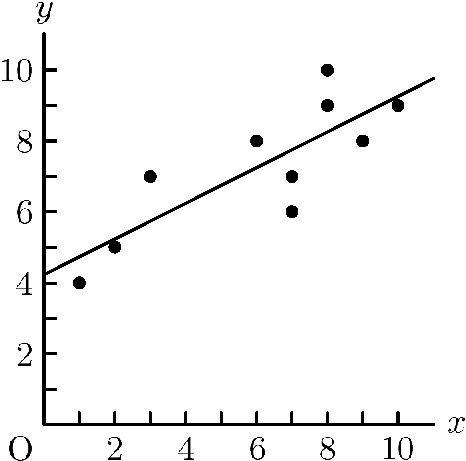
\includegraphics[scale = 0.5]{./figure/98.pdf}
			\end{figure}
		}
		\end{enumerate}
	}
	\item{
		\begin{enumerate}
			\item{
				平均 $\overline{x}$, $\overline{y}$ および $\overline{xy}$ はそれぞれ
				\begin{align}
					\overline{x} &= \frac{55.2 + \cdots + 89.7}{5} = 76.86, \\
					\overline{y} &= \frac{7.4 + \cdot + 0.3}{5} = 2.74, \\
					\overline{xy} &= \frac{55.2\cdot 7.4 + \cdot + 89.7\cdot 0.3}{5} = 180.45.
				\end{align}
				これより, $x$ と $y$ の共分散 $s_{xy}$ は
				\begin{align}
					s_{xy} = \overline{xy} - \overline{x}\cdot \overline{y} = 180.45 - 76.86\cdot 2.74 \simeq -30.15.
				\end{align}
				また, $x$ の分散 (標準偏差の 2 乗) ${s_{x}}^{2}$ は
				\begin{align}
					{s_{x}}^{2} &= \frac{(55.2 - 76.86)^{2} + \cdots + (7.4 - 2.74)^{2}}{5} \\
						&\simeq 147.17.
				\end{align}
				求める方程式を
				\begin{align}
					y = ax + b\quad (a, b\in \mathbb{R})
				\end{align}
				とおくと, 以上より
				\begin{align}
					a &= \frac{s_{xy}}{{s_{x}}^{2}} = -\frac{30.15}{147.17} \simeq -0.205, \\
					b &= \overline{y} - a\overline{x} = 2.74 - (-0.205)\cdot 76.86 \simeq 18.496.
				\end{align}
				すなわち, 求める方程式は
				\begin{align}
					\red{y = -0.205x + 18.496}.
				\end{align}
			}
			\item{
				(1) で求めた方程式に $x = 85$ を代入して
				\begin{align}
					y = -0.205\cdot 85 + 18.496 \simeq 1.1
				\end{align}
				より, \red{1.1\%}.
			}
		\end{enumerate}
	}
\end{qenumerate}